\fbox{\begin{minipage}{16.3cm}
\vspace{2mm}
P is a \textbf{transition probability matrix} if:
\begin{enumerate}
\item All of the entries are non-negative.
\item The sum of entries in each row is 1.
\end{enumerate}

\vspace{.8cm}

A \textbf{Markov chain} is defined by four things: (\state, $\pi_0$, 
$P$, $\{X_n\}_{n=0}^{\infty}$) \newline
\begin{center}
\begin{tabular}{l l}
\state & Set of states \\
$\pi_0$ & Initial probability distribution \\
$P$ & Transition probability matrix \\
$\{X_n\}_{n=0}^{\infty}$ & Sequence of random variables where: \\

& \hspace{5mm} $\P[X_0 = i] = \pi_0(i), i \in \state $ \\
& \hspace{5mm} $ \P[X_{n + 1} = j | X_n = i, X_{n-1}, \dotsc , X_0] = 
\P(i, j), \forall n \geq 0, \forall i, j \in \state $
\end{tabular}
\end{center}

\vspace{1cm}

A Markov chain is \textbf{irreducible} if we can go from any state to 
any other state, possibly in multiple steps.

\vspace{1cm}

Define value \textbf{$d(i)$} for each state $i$ as:
\[d(i) \coloneqq g.c.d\{n > 0 | P^n(i, i) = \P[X_n = i | X_0 = i] > 0 \}, 
i \in \state\]

If $d(i) = 1$, then the Markov chain is \textbf{aperiodic}. If $d(i) 
\neq 1$, then the Markov chain is periodic and its \textbf{period} is 
$d(i)$.

\vspace{1cm}

A distribution $\pi$ is \textbf{invariant} if $\pi \cdot P = \pi$.

\vspace{1cm}

\textbf{Theorem 24.3:} A finite irreducible Markov chain has a unique 
invariant distribution.
\textbf{Theorem 24.4:} All irreducible and aperiodic Markov chains 
converge to the unique invariant distribution. If a Markov chain is 
finite and reducible, the amount of time spent in each state approaches 
the invariant distribution as n grows large

Equations that model what will happen at the next step are called 
\textbf{first step equations}

\vspace{5mm}

\begin{minipage}[b]{0.6\linewidth}
\begin{center}
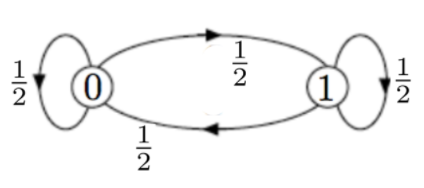
\includegraphics[width=4cm]{definitions_markov_chain.jpg} 
\end{center}
\end{minipage}%
\hfill
\begin{minipage}[b]{0.4\linewidth}
Denote $\beta(i, j)$ as the expected amount of time it would take to 
move from $i$ to $j$.
$\beta(0, 1) = 1 + \frac{1}{2} \cdot \beta(0, 1)$
$\beta(1, 1) = 0$

\end{minipage}

\end{minipage}}